\PassOptionsToPackage{hypertexnames=false}{hyperref}
\documentclass[a4paper,fleqn]{cas-sc}

\usepackage[authoryear,longnamesfirst]{natbib}
\usepackage{amsmath,amssymb,amsfonts}
\usepackage{graphicx}
\usepackage{booktabs}
\usepackage{multirow}
\usepackage{algorithm}
\usepackage{algpseudocode}
\usepackage{xurl}

% Anonymous-review placeholders. Replace only after the final author order and
% ORCID records have been approved by all authors.
\RenewDocumentCommand \printorcid {} {}

\newcommand{\breeze}{BREEZE}
\newcommand{\pucond}{N09\_M07\_F10}
% Generated by breeze/scripts/build_paper_tables.py; do not edit.
\newcommand{\BreezePUPassedTests}{12}
\newcommand{\BreezePUHolmBound}{0.001}
\newcommand{\BreezeCWRUPassedTests}{72}
\newcommand{\BreezeCWRURegisteredTests}{72}
\newcommand{\BreezeCWRUAccDeltaMin}{1.7}
\newcommand{\BreezeCWRUAccDeltaMax}{3.5}
\newcommand{\BreezeCWRUFOneDeltaMin}{1.9}
\newcommand{\BreezeCWRUFOneDeltaMax}{3.6}
\newcommand{\BreezeBerkeleyPassedTests}{15}
\newcommand{\BreezeBerkeleyRegisteredTests}{18}
\newcommand{\BreezeBerkeleyUnstructuredPassedTests}{12}
\newcommand{\BreezeBerkeleyUnstructuredRegisteredTests}{12}
\newcommand{\BreezeBerkeleyLowShotRuleEffectRange}{0.2--0.5}
\newcommand{\BreezeBerkeleyNTwoAccRuleDelta}{0.267}
\newcommand{\BreezeBerkeleyNFiveAccRuleDelta}{0.468}
\newcommand{\BreezeBerkeleyNFiveFOneRuleDelta}{0.407}
\newcommand{\BreezeBerkeleyNTenAccRuleDelta}{0.055}
\newcommand{\BreezeBerkeleyNTenFOneRuleDelta}{0.020}
\newcommand{\BreezePUHealthyReferenceN}{1200}
\newcommand{\BreezePUORReferenceN}{1202}
\newcommand{\BreezePUIRReferenceN}{1444}
\newcommand{\BreezeGlobalCoreHypotheses}{102}
\newcommand{\BreezeGlobalDecisionAgreement}{102}
\newcommand{\BreezeProposalSlotsPerClass}{150}
\newcommand{\BreezeTotalProposalSlots}{450}
\newcommand{\BreezeHealthyAdmissionRate}{60}
\newcommand{\BreezeORAdmissionRate}{60}
\newcommand{\BreezeIRAdmissionRate}{71}
\newcommand{\BreezeAdmissionKZeroCumulative}{205}
\newcommand{\BreezeAdmissionKOneCumulative}{241}
\newcommand{\BreezeAdmissionKTwoCumulative}{268}
\newcommand{\BreezeAdmissionKThreeCumulative}{286}
\newcommand{\BreezeAdmissionKOneIncrement}{36}
\newcommand{\BreezeAdmissionKTwoIncrement}{27}
\newcommand{\BreezeAdmissionKThreeIncrement}{18}
\newcommand{\BreezeAdmissionKThreeUnadmitted}{164}
\newcommand{\BreezePULOCOVOneFailures}{57}
\newcommand{\BreezePULOCOVTwoFailures}{60}
\newcommand{\BreezePULOCORegisteredTests}{96}
\newcommand{\BreezeMUTCMPassedTests}{2}
\newcommand{\BreezeMUTCMRegisteredTests}{6}


\begin{document}
\let\WriteBookmarks\relax
\def\floatpagepagefraction{1}
\def\textpagefraction{.001}

\shorttitle{BREEZE physics-verified LLM recipe admission}
\shortauthors{Author One et~al.}

\title[mode=title]{\breeze: Physics-Verified LLM Recipe Generation for
Few-Shot Condition Monitoring}

\author[1]{Author One}
\author[1]{Author Two}

\affiliation[1]{organization={Department},
  city={City},
  country={Country}}

\begin{abstract}
Scarce labelled faults make it costly to train and select a signal generator
for every machine and operating regime. We introduce \breeze, a training-free
workflow that separates LLM recipe proposal, seeded deterministic rendering,
and physical admission calibrated exclusively on the real training split. The
verifier records each gate decision, rejects failed candidates unchanged, and
uses structured failure reports for bounded resampling. On file-disjoint PU,
LLM recipes outperform matched rule and random open-loop recipes for Accuracy
and Macro-F1 at 5, 10, and 25 real windows per class; all
\BreezePUPassedTests{} registered comparisons pass Holm correction
($q<\BreezePUHolmBound$, 20 seeds), as do all \BreezeCWRUPassedTests{}
provenance-valid CWRU comparisons across within-load0 and held-out loads 1--3
(40 seeds). On case/run-disjoint Berkeley milling,
\BreezeBerkeleyPassedTests/\BreezeBerkeleyRegisteredTests{} comparisons pass,
including all \BreezeBerkeleyUnstructuredPassedTests{} against non-structured
baselines; its lower-shot LLM--rule advantage, class-conditional diagnostics,
and six failed PU cross-condition attempts delimit the evidence. A pass states
train-calibrated admissibility; these results establish auditable,
physics-verified LLM-guided admission for the stated few-shot protocols,
outside claims of formal physical validity, zero-data diagnosis, or universal
generator superiority.
\end{abstract}

\begin{keywords}
Condition monitoring \sep Large language model \sep Synthetic data \sep
Physics-verified admission \sep Few-shot diagnosis \sep Time-series generation
\end{keywords}

\maketitle

\section{Introduction}
\label{sec:intro}

Industrial fault diagnosis faces a structural data imbalance. Healthy
operation is abundant, whereas labelled faults are scarce, expensive to seed,
and rarely observed under every load and speed. New machines, sensor layouts,
and operating regimes therefore offer only a few examples of the events that a
diagnostic model must recognize.

Existing augmentation routes trade modelling capacity for target-data cost.
Conventional transformations are inexpensive, while VAEs, GANs, and diffusion
models can learn richer signal distributions through target-data training and
model selection~\citep{li2020augmentation,zhao2020vae,zhang2021semivae,
goodfellow2014gan,kingma2014vae,ho2020ddpm}. This investment is practical for a
large stable corpus, but becomes costly when each new deployment supplies only
a few labelled faults.

LLM-authored recipes create an inference-time alternative to target-specific
generator training. An LLM can express machine metadata, fault class, and
signal structure as a compact recipe, which a numerical renderer executes as a
waveform. This separation turns the language model into a proposal source and
keeps signal construction explicit.

The recipe interface also creates a reliability gap between valid syntax and
supported signal evidence. A well-formed recipe can still yield unsupported
amplitudes, implausible spectral allocation, missing fault-frequency evidence,
or repeated samples. Prompt instructions provide no deterministic basis for
deciding which candidates should enter a diagnostic training pool.

\breeze\ closes this gap through train-calibrated admission. The LLM proposes a
JSON recipe, a fixed renderer maps the recipe and seed to a waveform, and a
deterministic verifier evaluates gates calibrated from the corresponding outer
training split. Each rejection report identifies measured violations and
conditions a bounded resampling round, while the held-out test split remains
isolated from recipe construction and admission. Figure~\ref{fig:framework}
summarizes this closed loop.

\begin{figure*}
  \centering
  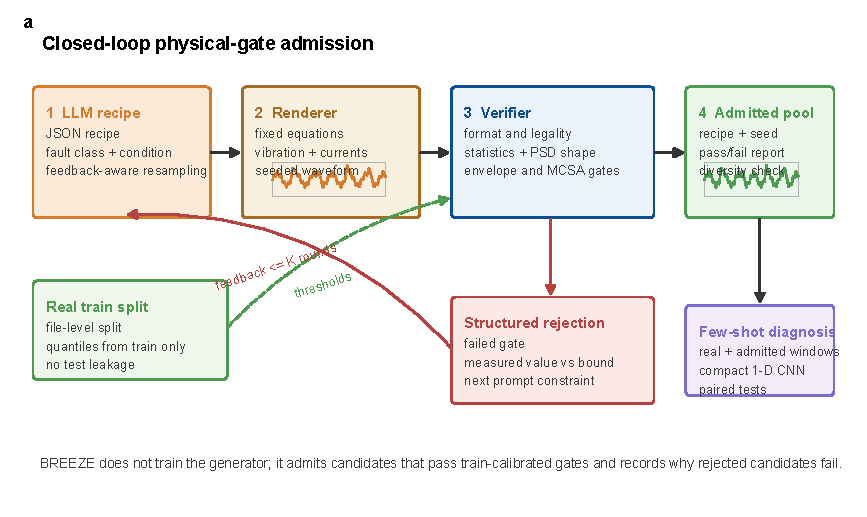
\includegraphics[width=\textwidth]{figs/framework.pdf}
  \caption{The \breeze\ workflow. The LLM proposes a structured recipe, a
  fixed seeded renderer constructs vibration and, when available, current
  channels, and a verifier calibrated exclusively on the real training split
  admits or rejects the candidate. A rejection becomes structured feedback
  for at most $K$ further rounds. Rejected signals are not repaired.}
  \label{fig:framework}
\end{figure*}

Three evaluation questions organize the evidence. First, does the LLM
contribute beyond random or engineer-written recipes under a matched renderer?
Second, do admitted signals exhibit train-supported time-domain, spectral,
envelope, and diversity evidence? Third, does the resulting pool provide stable
diagnostic utility under file-, load-, or experiment-disjoint few-shot
protocols? Paired source ablations, class-conditional diagnostics,
leakage-resistant splits, and corrected statistical tests answer these
questions together.

The paper makes four contributions:
\begin{enumerate}
  \item \textbf{Separate} LLM time-series generation into a
  recipe--renderer--verifier system, enabling independent auditing of language
  proposals, numerical signal construction, and train-calibrated admission.
  \item \textbf{Integrate} mixed physical gates---format legality, robust signal
  statistics, Welch-PSD shape, envelope-spectrum evidence, reliability-gated
  current evidence, and diversity---into a bounded rejection/resampling loop
  without training a target-data generator.
  \item \textbf{Establish} the contribution of LLM recipes under matched few-shot
  protocols on three public datasets: PU, CWRU, and Berkeley milling. The
  registered evidence comprises 20 PU seeds and 40 seeds for CWRU and Berkeley,
  with family-wise Holm correction.
  \item \textbf{Report} negative evidence as part of the method boundary: the full
  six-stage PU leave-one-condition-out (LOCO) failure chain, process-metadata
  confounding in UMich milling, and a stopped MU-TCM inner-validation line.
\end{enumerate}

The evidence supports a deliberately bounded admission claim. \breeze\ shows
that accepted candidates satisfy declared train-supported gates and improve
the stated few-shot tasks under their frozen protocols. It does not establish
zero-real-data operation, universal cross-condition morphology transfer,
formal physical correctness, or superiority to every learned generator.

\section{Related work and positioning}
\label{sec:related}

\subsection{Time-series generation for diagnosis}

Trainable models dominate general time-series generation. Their architectures
include recurrent conditional GANs, TimeGAN, transformer GANs, variational
models, and diffusion models~\citep{esteban2017rcgan,yoon2019timegan,
li2022ttsgan,li2022ttscgan,liao2020sigcwgan,desai2021timevae,
nichol2021improved,kong2021diffwave,tashiro2021csdi,alcaraz2022sssd,
rasul2021timegrad}. Machinery-specific variants address scarce or imbalanced
signals through sparsity constraints, deep feature-enhanced filtering,
frequency learning, spectrum-guided sampling, and FillingGAN
\citep{ma2021scgan,liu2022dfegan,ko2023flgn,kim2024sgan,lin2025fillinggan}.
\breeze\ differs by evaluating structured recipe generation at an operating
point without target-generator optimization.

\subsection{Physics-informed generation}

Physics-informed generation embeds equations, mechanisms, or physical penalties
in a trainable model~\citep{raissi2019pinn}. Recent rotating-machinery GAN and
diffusion systems encode impact response, speed modulation, multimodal
features, or condition embeddings~\citep{gao2025physicsgan,
liu2026physicsdiffusion,guo2025diffucd}. These models can learn their physical
objectives through target-data optimization, followed by generator selection.

Generated-data filtering provides a complementary control mechanism. DFE-GAN
and SGAN-DDS show that selection and diversity control affect the final
pool~\citep{liu2022dfegan,kim2024sgan}. \breeze\ differs by placing mixed
bearing-diagnostic gates, train-only calibration, structured feedback, and
per-sample audit records inside deterministic inference-time admission.

\subsection{LLMs and machinery signals}

LLMs provide emerging interfaces to time-series and machinery knowledge. They
have been reprogrammed for forecasting without task-specific training, used as
numerical forecasters, and supplied with machinery priors for bearing health
management~\citep{jin2024timellm,gruver2023llmtime,peng2025bearllm}. BearGen is
the closest signal-generation study: an LLM produces signal descriptions that
condition a diffusion generator trained across multiple bearing datasets
\citep{lee2026beargen}. \breeze\ differs by asking the LLM for a structured
numerical recipe and executing it with a fixed renderer whose target-data path
has no learned weights.

\begin{table*}[t]
\centering
\caption{Positioning against representative synthetic-signal systems. ``Target
training'' denotes optimization of a generator on the target signal corpus.}
\label{tab:positioning}
\small
\setlength{\tabcolsep}{4pt}
\begin{tabular}{@{}p{2.2cm}p{3.0cm}p{1.8cm}p{2.3cm}p{4.0cm}@{}}
\toprule
Method family & Generative mechanism & Target training & Physical control & Primary evidence pattern \\
\midrule
DFE-GAN / SGAN-DDS & Learned adversarial generator plus filtering or sampling & Yes & Learned features and spectrum guidance & Fidelity, diversity, and diagnosis \\
Physics-informed GAN / diffusion & Learned generator with physical priors or condition embedding & Yes & Training loss or architecture & Mechanism, multidomain fidelity, diagnosis \\
BearGen & LLM descriptions condition a learned diffusion model & Yes & Description guidance and learned denoising & Eight bearing datasets, quality, few-shot, cost \\
\breeze & LLM JSON recipe plus fixed seeded renderer & No & Train-calibrated admission and rejection & Source ablation, gate reports, physical distances, paired diagnosis \\
\bottomrule
\end{tabular}
\end{table*}

\subsection{Diagnostic observables used as gates}

Established diagnostic observables expose complementary aspects of
rolling-element faults. Envelope analysis, spectral kurtosis, and the fast
kurtogram reveal stochastic or pseudo-cyclostationary impacts
\citep{randall2011bearing,antoni2006spectral,antoni2007kurtogram}, while Welch
PSD estimation represents spectral shape~\citep{welch1967psd}. Motor-current
sidebands add bearing evidence when the real training data support class
separability~\citep{schoen1995mcsa}. \breeze\ differs by converting these
observables into explicit, train-calibrated admission gates.

\section{Problem formulation and framework}
\label{sec:method}

\subsection{Train-calibrated admission}

Reliable admission requires a decision rule calibrated entirely within the
outer training split. Let
$\mathcal{D}_{\mathrm{tr}}=\{(x_i,y_i,m_i)\}_{i=1}^{n}$ denote its real
windows, class labels, and available machine metadata. For requested class $y$
and condition $m$, the LLM proposes recipe $r_t$ at feedback round $t$. The
following mapping makes recipe execution and local randomness explicit:
\begin{equation}
  \tilde{x}_{t,s}=R(r_t,m;s),
\end{equation}
where the seeded renderer $R$ archives $s$ with the recipe. The verifier then
maps the rendered waveform to both an admission decision and its evidence
report:
\begin{equation}
 (a_{t,s},q_{t,s})=V(\tilde{x}_{t,s},y,m;\mathcal{D}_{\mathrm{tr}}),
 \qquad a_{t,s}\in\{0,1\}.
 \label{eq:verifier}
\end{equation}
Equation~\eqref{eq:verifier} exposes the decision $a_{t,s}$ and the diagnostic
report $q_{t,s}$ as separate outputs. Renderer inputs, gate calibration,
feedback, and pool selection all remain confined to the outer training split.

Admission must represent interval support, one-sided evidence, healthy
suppression, and diversity in one decision. For deterministic feature $f_j$,
class-supported bounds $[l_{j,y,m},u_{j,y,m}]$, healthy fault-prominence score
$p_f$, physical embedding $e(x)$, and current admitted set $\mathcal{S}_y$, the
following system shows the four predicate types:
\begin{align}
 l_{j,y,m}\leq f_j(x)\leq u_{j,y,m} &\quad\text{(interval)},\nonumber\\
 f_j(x)\leq u_{j,y,m}\ \text{or}\ f_j(x)\geq l_{j,y,m}
   &\quad\text{(one-sided evidence)},\nonumber\\
 p_f(x)\leq u_{f,\mathrm{healthy}}
   &\quad\text{(healthy suppression)},\nonumber\\
 \min_{z\in\mathcal{S}_y}\lVert e(x)-e(z)\rVert_2\geq\delta_y
   &\quad\text{(diversity)}.
 \label{eq:mixed-gates}
\end{align}
The intersection of the active predicates defines the admissible set.
Membership therefore records compliance with the configured gates under their
training calibration.

\subsection{Responsibility boundaries}

Attributing an observed gain requires explicit boundaries between proposal,
waveform construction, admission, and diagnosis. Figure~\ref{fig:boundary}
assigns one component to each responsibility. The LLM selects recipe fields,
the renderer enforces the signal equations, the verifier measures compatibility
with train-supported evidence, and the downstream classifier measures utility.
Matched source comparisons can then isolate the recipe source while holding the
other components fixed.

\begin{figure*}
  \centering
  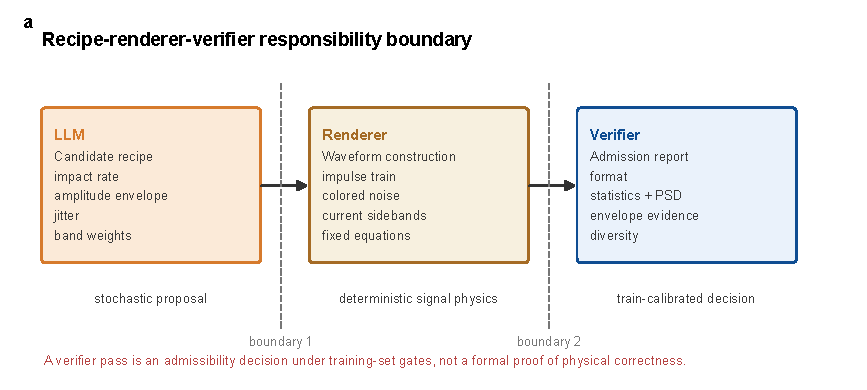
\includegraphics[width=\textwidth]{figs/responsibility_boundary.pdf}
  \caption{Component responsibility boundary. The LLM selects recipe
  parameters; the renderer alone constructs waveforms; the verifier admits or
  rejects without repair; and the classifier is used only for downstream
  evaluation. Every formal source comparison holds renderer and classifier
  fixed.}
  \label{fig:boundary}
\end{figure*}

The structured recipe exposes every LLM-controlled degree of freedom. It
records shaft and fault frequencies, target RMS, periodic-impact rate,
amplitude, decay, resonance, slip jitter, amplitude variation, load-zone
modulation, background components, random machine transients, eight
vibration-band weights, and optional two-phase current parameters. The initial
prompt supplies class, condition metadata, bearing kinematics, a
training-derived exemplar description, and the JSON schema. The feedback
prompt adds the previous recipe, each measured gate violation, its supported
bound, and a request for proportional parameter change. Complete prompt
builders and schemas are preserved in \texttt{src/llm.py}.

\subsection{Seeded renderer}

A fixed renderer is needed to compare recipe sources under identical waveform
construction. For PU vibration, the renderer combines deterministic background
harmonics, Poisson machine transients, a jittered train of resonant impacts,
and band-shaped noise. The equations expose the source terms and the link
between impact interval and requested fault frequency:
\begin{align}
x_v(t)={}&\sum_q A_q\sin(2\pi f_qt+\phi_q)
 +\sum_{\ell} b_{\ell}h(t-u_{\ell})
 +\sum_k a_kh(t-t_k)+\epsilon_b(t),\label{eq:vibration}\\
h(\tau)={}&\mathbf{1}_{\tau\geq0}\exp(-\tau/\tau_d)
             \sin(2\pi f_r\tau+\phi),\label{eq:impact}\\
t_{k+1}-t_k={}&f_f^{-1}(1+\xi_k).
\end{align}
Here $u_\ell$ follows a Poisson background process, $f_f$ is the requested
fault frequency, and $\xi_k$ is bounded recipe jitter. Inner-race impact
amplitudes may be modulated at shaft frequency. The renderer shapes additive
noise over the fixed eight-band grid and applies the same deterministic target-
RMS normalization to every recipe source before admission. Both operations
belong to $R$ and precede the gate decision.

When two phase currents are available, the following equation makes carrier,
fault modulation, harmonics, and channel noise explicit for channel $p$:
\begin{align}
i_p(t)={}&A_p\bigl[1+\beta\cos(2\pi f_ft+\psi)\bigr]
\left[\sin(2\pi f_et+\phi_p)
+\sum_{h\in\{3,5,7\}}\rho_h\sin(2\pi hf_et+\phi_{p,h})\right]
+\eta_p(t),
\label{eq:current}
\end{align}
where $f_e$ is supply frequency. The code and archived seed make $R(r,m;s)$
deterministic.

Berkeley requires a dataset-specific milling renderer under the same component
responsibility principle. Its multichannel renderer starts from a train-only
channel exemplar, adds the recipe's transient and band-energy structure, and
preserves channel-specific location and scale. This renderer is calibrated
inside the outer training fold, while
Eqs.~\eqref{eq:vibration}--\eqref{eq:current} define the bearing-channel model.

\subsection{Verifier gates}

Reliable pool construction requires evidence beyond recipe legality, so the
verifier evaluates six complementary gate families:
\begin{enumerate}
  \item \textbf{Legality:} exact shape, finite samples, non-degenerate
  channels, and absence of long repeated runs.
  \item \textbf{Robust statistics:} class- and channel-conditional RMS,
  standard deviation, peak, kurtosis, skewness, and crest factor inside
  train-derived quantile or robust-union domains.
  \item \textbf{Spectral shape:} triangular-band Welch-PSD fractions and
  PSD-CDF Wasserstein-1 distance to the class training reference.
  \item \textbf{Envelope evidence:} resonance-band Hilbert demodulation,
  prominence near the requested BPFO, BPFI, BSF, or FTF frequency, harmonic support,
  and suppression of unsupported peaks for healthy candidates.
  \item \textbf{Current evidence:} vector-current sideband scores become active
  when training data establish class separability; otherwise they remain
  audit-only measurements.
  \item \textbf{Diversity:} a lower nearest-neighbour bound in the physical
  feature embedding relative to a train-derived real--real reference.
\end{enumerate}
PU training data leave the MCSA score audit-only. Current-signature consistency
is therefore reported only for pools whose training split activates that gate.

\subsection{Closed-loop construction and audit records}

Closed-loop admission must bound proposal cost while preserving every decision
needed for audit and replay. Algorithm~\ref{alg:loop} states this contract for
one proposal slot.

\begin{algorithm}[t]
\caption{\breeze\ recipe admission for one proposal slot}
\label{alg:loop}
\begin{algorithmic}[1]
\Require class $y$, condition $m$, LLM $G$, renderer $R$, verifier $V$,
round limit $K$, renderer seeds $\mathcal{S}$
\State $q_{-1}\gets\varnothing$
\For{$t=0$ to $K$}
  \State $r_t\gets G(y,m,q_{t-1})$
  \ForAll{$s\in\mathcal{S}$}
    \State $\tilde{x}_{t,s}\gets R(r_t,m;s)$
    \State $(a_{t,s},q_{t,s})\gets V(\tilde{x}_{t,s},y,m)$
    \If{$a_{t,s}=1$}
      \State archive recipe, seed, waveform hash, and full gate report
      \State \Return admitted slot and all diversity-admitted windows
    \EndIf
  \EndFor
  \State $q_t\gets\mathrm{AggregateFailures}(\{q_{t,s}\})$
\EndFor
\State \Return rejected slot with terminal failure report
\end{algorithmic}
\end{algorithm}

A \emph{slot} is one requested class-conditioned recipe unit, whereas a
\emph{window} is the $C\times N$ tensor supplied to the classifier. One slot
can archive candidates from several feedback rounds, and its admitted recipe
can be rendered with several deterministic seeds. The frozen pipeline renders
three seeds per recipe and can retain additional diversity-admitted expansions,
so one admitted slot can yield multiple windows. This distinction matters
because slot counts measure LLM proposal cost, while window counts measure the
classifier's augmentation budget.

Generation provenance determines which stages can be replayed exactly. The
CWRU archive records the OpenAI-compatible model identifier
\texttt{mimo-v2.5}, temperature 0.8, top-$p$ 0.9, and maximum 900 output
tokens, although the provider did not expose sampling seeds. The earlier PU
archive preserves prompts, recipes, rendered pools, and local seeds; its
original provenance record omits the exact provider version and top-$p$.
Consequently, the frozen PU pools are reproducible from archived recipes and
renderer seeds, while exact regeneration of the original language responses
remains unavailable. Manuscript assembly required no new LLM call.

\section{Experimental design}
\label{sec:setup}

\subsection{Public datasets and leakage-resistant splits}

Leakage-resistant evaluation requires splitting acquisition units before
sampling windows. The formal evidence uses the established PU and CWRU bearing
benchmarks~\citep{lessmeier2016pu,smith2015cwru} and Berkeley milling from the
NASA prognostics repository~\citep{agogino2007milling}. Their file-, load-, or
case/run-level protocols appear in Table~\ref{tab:datasets}, and only these
grouped splits support formal claims.

\begin{table*}[t]
\centering
\caption{Formal datasets and frozen protocols. Counts are windows after the
declared split.}
\label{tab:datasets}
\small
\setlength{\tabcolsep}{4pt}
\begin{tabular}{@{}p{1.4cm}p{2.0cm}p{2.2cm}p{2.8cm}p{1.7cm}p{3.5cm}@{}}
\toprule
Dataset & Sampling and input & Classes & Operating regime & Train/test & Split unit \\
\midrule
PU & 8 kHz, 3 channels, 2048 samples & healthy, OR, IR & \pucond: 900 rpm, 0.7 Nm, 1000 N & 3846/962 & chronological measurement files within bearing; zero shared file/window keys \\
CWRU & 12 kHz drive-end vibration, 2048 samples & healthy, IR, ball, OR & motor loads 0--3; defects 0.007--0.028 in & 696/306 for within-load0 & chronological within-file for load0; loads 1--3 held out separately for clean transfer tests \\
Berkeley & 250 Hz, 6 channels, 512 samples & healthy ($VB<0.2$), degraded ($VB\geq0.2$) & feed, depth, and material combinations & 1836/646 & disjoint machining case/run groups \\
\bottomrule
\end{tabular}
\end{table*}

The PU protocol isolates measurement files within each bearing. Its healthy,
OR, and IR classes contain 1200, 1202, and 1444 training windows, together with
300, 301, and 361 test windows. The input retains one vibration and two
phase-current channels.

The CWRU protocol tests both within-load diagnosis and source-load transfer. It
evaluates a within-load0 split and three folds that hold out load1, load2, or
load3. The frozen synthetic pools derive from load0, which belongs to the
training side of these three folds. Reusing these pools gives the archived
held-out-load0 fold target-load provenance, so that fold remains an audit
artifact.

The Berkeley protocol isolates machining case/run groups before windowing. Its
six channels contain spindle AC and DC current, table and spindle vibration,
and table and spindle acoustic emission. Train-only inner validation fixed the
healthy/degraded threshold and split before the one-time 40-seed formal run.

\subsection{Recipe-source and augmentation controls}

Testing the LLM contribution requires changing the proposal source while
holding every downstream factor fixed. The central ablation therefore retains
the applicable renderer, data split, synthetic budget, CNN, and paired seeds:
\begin{itemize}
  \item \textbf{LLM + verifier:} class- and condition-aware JSON recipe,
  physical admission, and bounded feedback.
  \item \textbf{Rule + verifier:} engineer-written class template with
  train-supported parameter ranges, the same renderer, and the same verifier;
  no LLM call.
  \item \textbf{Random open-loop:} random legal recipe values rendered without
  feedback. On PU this is the matched non-semantic downstream control; a
  separate random-recipe verifier audit is also reported.
  \item \textbf{Noise augmentation:} real few-shot windows with channel-scaled
  jitter and amplitude scaling, using the same synthetic count.
  \item \textbf{Real only:} the paired few-shot subset without synthetic data.
\end{itemize}
The completed formal families match these controls to each dataset. CWRU
compares LLM with rule, noise, and real only over within-load0 and held-out
loads 1--3. Berkeley adds random open-loop, while PU Phase-A focuses on LLM
versus rule and random open-loop.

The available baseline archive fixes the quantitative comparison boundary.
Checkpointed TimeGAN and 1-D DDPM implementations reached smoke/development
output before a completed predeclared formal run, which excludes them from the
quantitative claims. Superiority to trained GAN or diffusion methods therefore
awaits a matched formal run. FID/KID-style learned distances also remain
unreported because the protocol lacks a fixed, validated domain feature
extractor; their general role is described by
\citet{heusel2017fid,binkowski2018mmdgan}.

\subsection{Few-shot classifier and statistical protocol}

Matched downstream evaluation requires a fixed classifier and paired sources of
randomness. All methods within a dataset therefore share the same compact 1-D
CNN. Its three convolution blocks use 16, 32, and 64 channels, kernels 15, 9,
and 5, stride two, max-pooling after the first two blocks, adaptive average
pooling to length eight, and a linear classifier. Adam uses learning rate
$3\times10^{-4}$, weight decay $10^{-4}$, batch size 32, and cross-entropy
loss. PU uses 60 epochs; the frozen CWRU and Berkeley protocols use 20.
Training-channel mean and standard deviation normalize both train and test
data.

The dataset-specific budgets define the registered comparison cells. PU uses
$n_{\mathrm{real}}\in\{5,10,25\}$, 150 synthetic windows per class, and 20
paired seeds. CWRU uses the same shot counts, 20 synthetic windows per class,
and 40 seeds. Berkeley uses $n_{\mathrm{real}}\in\{2,5,10\}$, 20 synthetic
windows per class, and 40 seeds. Accuracy and Macro-F1 are primary, while each
paired seed selects the same real subset and classifier initialization for
every method in its cell.

Registered inference preserves the pairing used in training. One-sided
Wilcoxon signed-rank tests compare paired seeds~\citep{wilcoxon1945paired}, and
Holm correction controls family-wise error within each predeclared comparison
family~\citep{holm1979multiple}. Benjamini--Hochberg values remain secondary
audit output, while the registered decision follows Holm
\citep{benjamini1995fdr}. We report direction, adjusted decision, seed count,
and the complete pass pattern. An unadjusted $p$ value near 0.05 remains
descriptive; significance requires the adjusted Holm decision.

\subsection{Physical and distribution diagnostics}

Physical and distribution diagnostics complement downstream accuracy by
measuring how each class relates to its outer-training reference. They include
RMS, kurtosis, skewness, crest factor, peak value, BPFO/BPFI/BSF/FTF peak
alignment where applicable, envelope prominence and harmonic support, PSD-CDF
Wasserstein-1 distance, relative band-energy error, and nearest-neighbour
distance. Wasserstein distance follows the optimal-transport interpretation of
\citet{villani2009transport}. The archived feature audit retains MMD with an RBF
kernel and median pairwise-distance bandwidth~\citep{gretton2012mmd}, while the
main figure reports directly interpretable distances. The core evidence uses
these direct diagnostics; t-SNE, UMAP, and Mixup remain outside the frozen
formal comparison~\citep{zhang2018mixup}.

\section{Results}
\label{sec:results}

\subsection{LLM recipes outperform rule and random sources on PU}

LLM recipes outperform rule and random open-loop recipes at every registered
PU shot count for both diagnostic metrics. All \BreezePUPassedTests{}
pairwise tests pass Holm correction ($q<\BreezePUHolmBound$), and
Table~\ref{tab:pu-phasea} reports the paired protocol means and standard
deviations.

\input{generated/pu_phasea.tex}

Seed-level deltas confirm that the PU LLM advantage is positive across every
registered source comparison for Accuracy and Macro-F1.
Figure~\ref{fig:downstream} shows these paired deltas alongside their
distributions. The matched design attributes this contribution to recipe
selection within the complete \breeze\ pipeline; the renderer and verifier
retain responsibility for waveform construction and admission.

\begin{figure*}
  \centering
  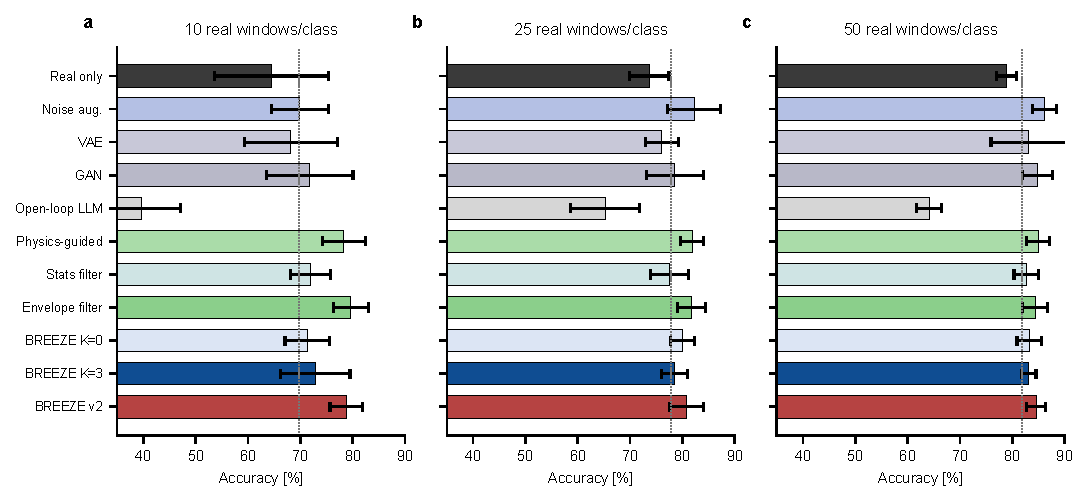
\includegraphics[width=\textwidth]{figs/downstream_bars.pdf}
  \caption{Paired downstream deltas. Points are seed-level differences; thick
  segments show interquartile ranges and diamonds show medians. (a) PU LLM
  minus rule or random open-loop. (b) CWRU within-load0 LLM minus rule or noise
  augmentation. (c) Berkeley LLM minus rule or noise augmentation. The dashed
  line is zero.}
  \label{fig:downstream}
\end{figure*}

\subsection{Load0-derived LLM recipes outperform comparators within load0 and
on held-out loads 1--3}

Load0-derived LLM recipes outperform every registered comparator within load0
and on provenance-valid held-out loads 1--3. The within-load0 means exceed rule
and noise augmentation at each shown shot count (Table~\ref{tab:cwru}), while
the combined protocol yields
\BreezeCWRUPassedTests/\BreezeCWRURegisteredTests{} positive Holm-corrected
LLM--comparator decisions. Figure~\ref{fig:cross} reports the source-load0
LLM--rule transfer deltas: Accuracy improves by \BreezeCWRUAccDeltaMin{} to
\BreezeCWRUAccDeltaMax{} percentage points, and Macro-F1 by
\BreezeCWRUFOneDeltaMin{} to \BreezeCWRUFOneDeltaMax{} points across shots and
held-out loads 1--3.

\input{generated/cwru.tex}

This result establishes source-load0 cross-load diagnostic utility for the
tested held-out loads 1--3. A strict four-fold LOLO and cross-bearing scope
remain outside this result because the reused synthetic pool gives the archived
held-out-load0 fold target-load provenance.

\subsection{LLM recipes beat non-structured Berkeley controls and provide a
qualified lower-shot advantage over rules}

LLM recipes beat the non-structured Berkeley controls in all
\BreezeBerkeleyUnstructuredPassedTests{} registered comparisons. Against the
strong structured rule reference, Accuracy passes at
$n_{\mathrm{real}}=2$, while the two-shot Macro-F1 comparison remains outside
the Holm decision; both metrics pass at $n_{\mathrm{real}}=5$. At
$n_{\mathrm{real}}=10$, the LLM and rule results converge and both registered
comparisons fall outside the Holm decision. This complete pattern yields
\BreezeBerkeleyPassedTests{} of \BreezeBerkeleyRegisteredTests{} passes, with
means reported in Table~\ref{tab:berkeley}.

\input{generated/berkeley.tex}

The Berkeley pattern localizes the additional LLM contribution to lower-shot
settings. The rule recipe supplies a demanding structured reference, and its
convergence with the LLM at ten shots shows that the additional LLM advantage
narrows as the real sample count increases. The registered table supports this
qualified source comparison within the binary Berkeley protocol, outside a
generic milling state-of-the-art scope.

\subsection{PU diagnostics show complementary physical agreement and non-copy
behaviour}

PU diagnostics show that admitted LLM pools combine class-relevant waveform
evidence with non-duplicate nearest-neighbour distances. Under the same fixed
demodulation procedure, Fig.~\ref{fig:waves} compares real, LLM, rule, and
random windows. Admitted LLM and rule recipes preserve impulsive and envelope
structure more consistently than the random control while retaining visible
stochastic variation. These traces illustrate the population-level
distributions in Figs.~\ref{fig:boxplots}--\ref{fig:distances}.

\begin{figure*}
  \centering
  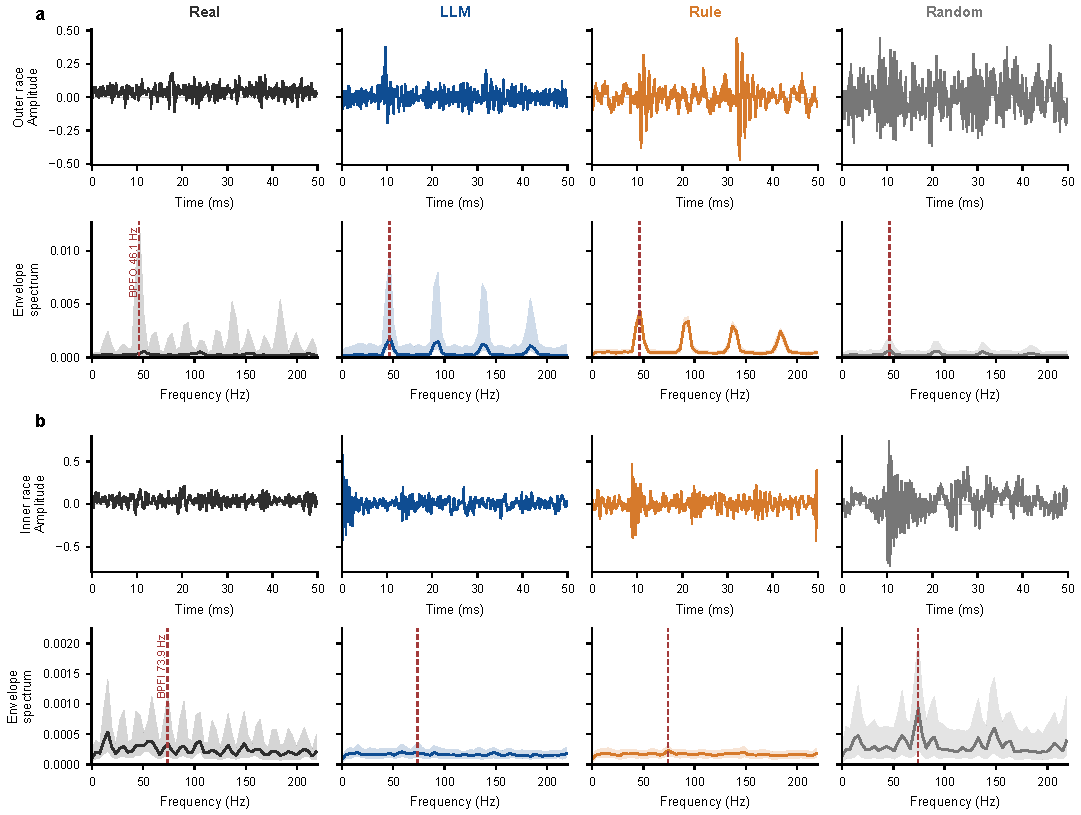
\includegraphics[width=\textwidth]{figs/waveforms.pdf}
  \caption{PU waveform and envelope-spectrum comparison. Rows are healthy,
  outer-race, and inner-race classes; columns compare real training, LLM,
  rule, and random open-loop windows. All envelope spectra use the same fixed
  500--2000 Hz demodulation band. Vertical markers denote the class-relevant
  kinematic frequency.}
  \label{fig:waves}
\end{figure*}

\begin{figure*}
  \centering
  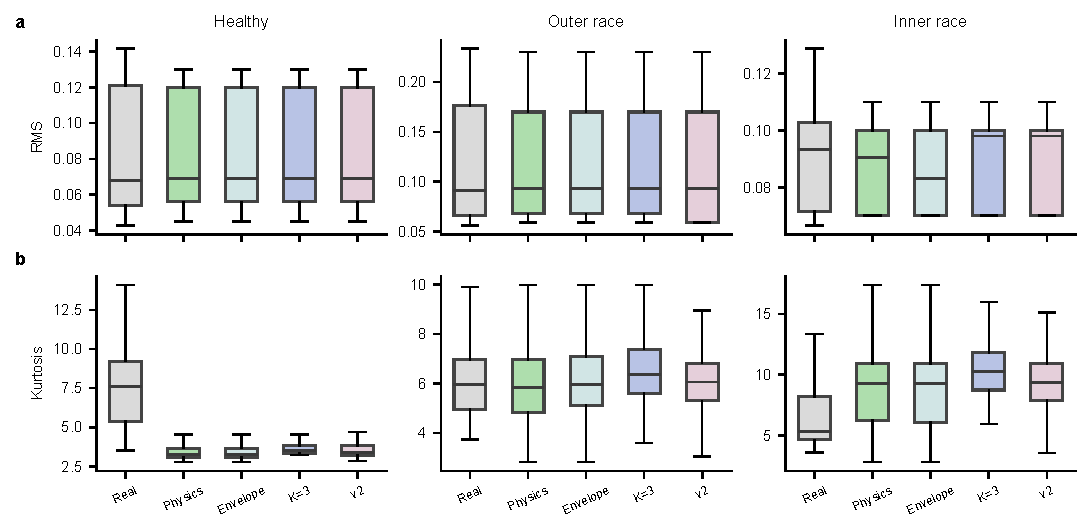
\includegraphics[width=\textwidth]{figs/boxplots.pdf}
  \caption{Class-conditional RMS and kurtosis distributions for the real PU
  training split and matched synthetic pools. Boxes show the frozen pool
  distributions; admission narrows unsupported statistical excursions without
  forcing equality to a single reference value.}
  \label{fig:boxplots}
\end{figure*}

\begin{figure*}
  \centering
  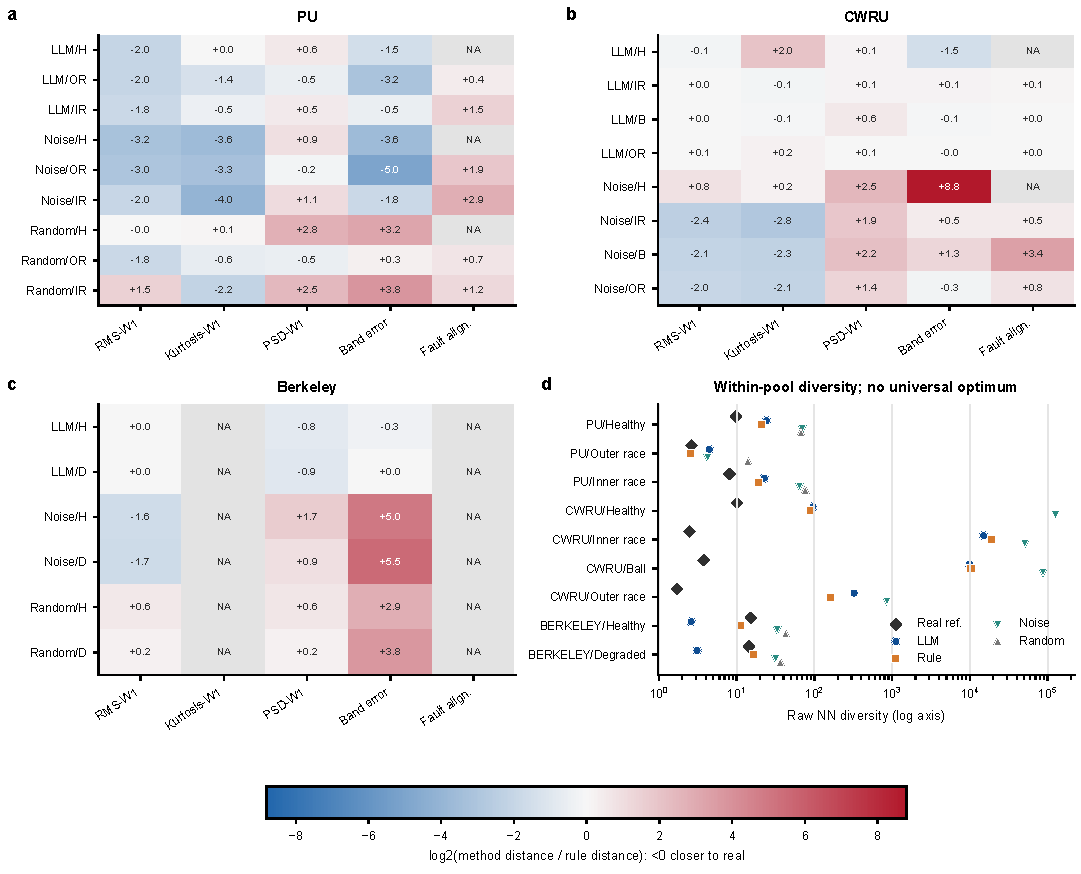
\includegraphics[width=\textwidth]{figs/metric_distances.pdf}
  \caption{Class-averaged physical diagnostics on PU, CWRU, and Berkeley.
  Cells contain raw RMS Wasserstein-1, PSD-CDF Wasserstein-1, relative
  band-energy error, and nearest-neighbour diversity values; colour is scaled
  within each dataset and metric only. NA denotes a pool that does not exist in
  the frozen archive, not an imputed value. Diversity has no universally
  optimal direction.}
  \label{fig:distances}
\end{figure*}

Class-averaged PU distances favour LLM recipes over the matched recipe sources
on PSD, band energy, and RMS. Table~\ref{tab:physics} reports lower LLM PSD
distance and band-energy error than rule and random open-loop, together with
lower RMS distance than both recipe sources. Noise augmentation is closest in
RMS and band energy because it directly perturbs real windows. The LLM
nearest-neighbour distance also separates the pool from its closest real
reference under the frozen feature metric. This diversity value requires joint
interpretation with fidelity because arbitrarily large distances can indicate
unrealistic samples.

\input{generated/physics.tex}

External downstream tests, matched source controls, train/test separation, and
failed cross-condition experiments provide evidence beyond the shared physical
features. The prompt, renderer, and verifier encode some of the same bearing
quantities, which makes gate compliance necessary but insufficient evidence of
real-world physics.

\subsection{Closed-loop admission exposes proposal yield and class-specific
failure mechanisms}

Closed-loop accounting separates proposal cost from the downstream
augmentation budget. PU requests \BreezeProposalSlotsPerClass{} proposal slots
per class; Fig.~\ref{fig:acceptance}(a) reports archived round candidates,
panel (b) separates proposal slots, admitted slots, and kept rendered windows,
and panel (c) compares recipe sources. At $K=3$, the LLM process admits
\BreezeHealthyAdmissionRate\%, \BreezeORAdmissionRate\%, and
\BreezeIRAdmissionRate\% of healthy/OR/IR slots.

Recipe source determines whether the verifier can construct a balanced pool.
The random-recipe audit admits no slot, whereas rule admission varies by class.
This contrast makes the fixed rule a meaningful but incomplete substitute for
LLM proposal under the PU verifier.

\begin{figure*}
  \centering
  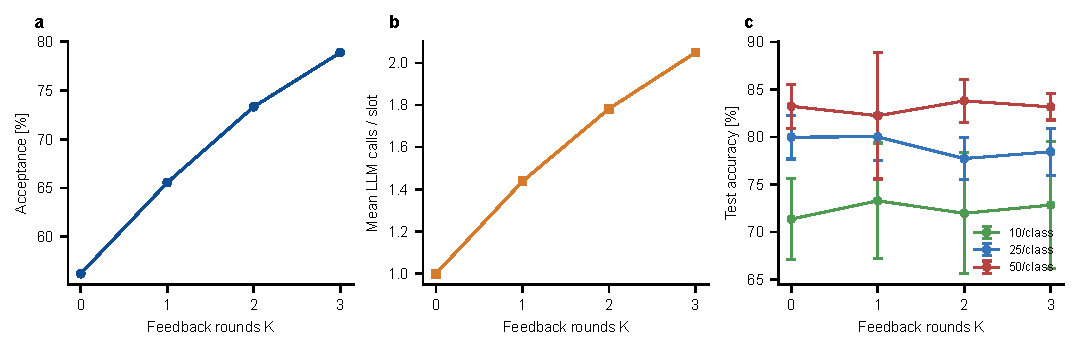
\includegraphics[width=\textwidth]{figs/acceptance_k.pdf}
  \caption{PU proposal accounting. (a) Number of archived candidates per
  proposal slot. (b) One-to-many mapping from
  \BreezeProposalSlotsPerClass{} class slots to admitted slots
  and diversity-kept windows. (c) Verifier slot-admission rates for LLM, rule,
  and random recipes. Random open-loop remains a downstream control; random
  recipes subjected to the verifier produce no balanced admitted pool.}
  \label{fig:acceptance}
\end{figure*}

Terminal failures reveal class- and source-specific rejection mechanisms.
Figure~\ref{fig:failreasons} reports the non-exclusive rates. Random recipes
fail statistical and spectral gates much more often than cached LLM recipes.
Healthy LLM candidates are rejected most often for unsupported envelope
evidence, whereas fault candidates more often violate the robust statistical
domain. A slot may fail several gates, so the percentages are non-additive.
The same report supplies the next feedback round with each measured violation
and its bound.

\begin{figure*}
  \centering
  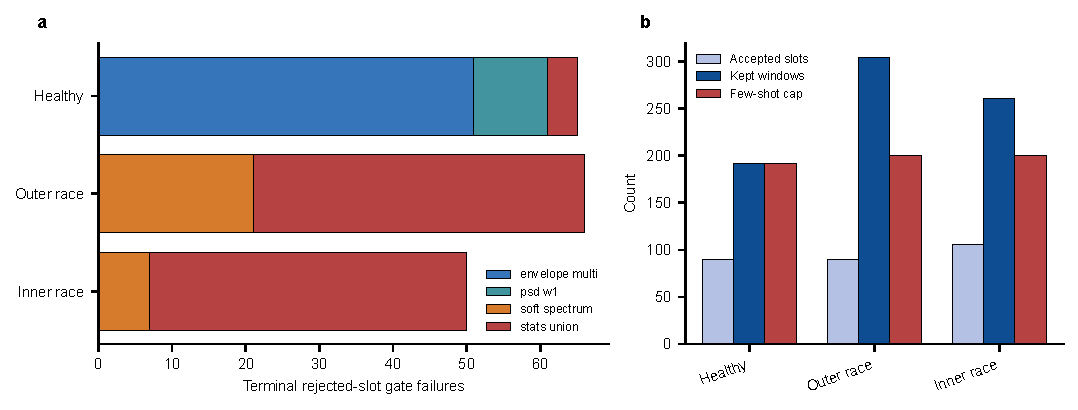
\includegraphics[width=\textwidth]{figs/failure_reasons.pdf}
  \caption{Non-exclusive PU gate-failure rates by class and recipe source.
  (a) Cached LLM $K=3$ rescreen. (b) Random recipes passed through the same
  verifier. Statistics, soft-spectrum, PSD-W1, and multi-band envelope failures
  are computed from frozen slot reports.}
  \label{fig:failreasons}
\end{figure*}

\section{Cross-condition evidence and negative results}
\label{sec:boundaries}

These failures define the method's applicability, and their protocol value is
to prevent unsupported extrapolation from positive within-condition results.

\subsection{CWRU load transfer succeeds while PU LOCO remains a failed stress
test}

CWRU source-load0 recipes transfer to the tested loads 1--3, whereas the PU
LOCO protocol remains unsuccessful. Figure~\ref{fig:cross} places these outcomes
side by side: PU v1 fails
\BreezePULOCOVOneFailures/\BreezePULOCORegisteredTests{} registered cells, and
v2 fails \BreezePULOCOVTwoFailures/\BreezePULOCORegisteredTests{}. The PU
failures cluster by held-out condition and persist across Accuracy, Macro-F1,
and shot counts, locating the unresolved boundary in condition-dependent
morphology.

\begin{figure*}
  \centering
  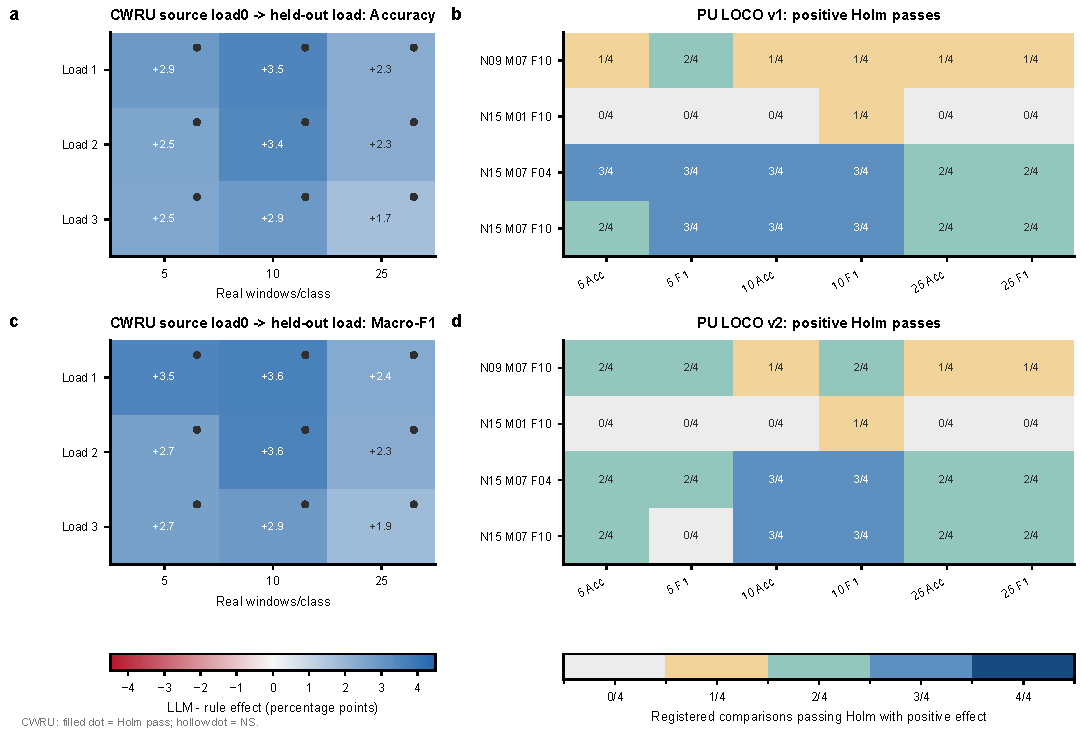
\includegraphics[width=\textwidth]{figs/cross_condition_heatmap.pdf}
  \caption{Cross-condition evidence. (a,c) CWRU LLM--rule Accuracy and
  Macro-F1 deltas when load0-derived pools are evaluated on held-out loads
  1--3. The archived held-out-load0 fold is excluded for target-load
  provenance. (b,d) Number of passed PU LOCO tests out of four registered
  comparisons in each condition--shot--metric cell for v1 and v2.}
  \label{fig:cross}
\end{figure*}

The six-stage PU audit localizes this boundary from kinematics through
source-only evidence (Fig.~\ref{fig:failurechain}). v1 exposed a kinematic
mismatch, and v2 corrected frequency handling while downstream performance
remained unsuccessful. v3 stopped when train-condition morphology mapping
could not form an admissible balanced pool. v4 stopped after both train-only
candidate-pool strategies failed admission, and v5 showed that its candidate
criterion also admitted wrong-label/noise controls. v6 stopped because
source-only cyclostationary coherence failed to separate all four held-out
targets. The formal held-out evaluations are v1 and v2; v3--v6 remain
development or admission stops.

\begin{figure*}
  \centering
  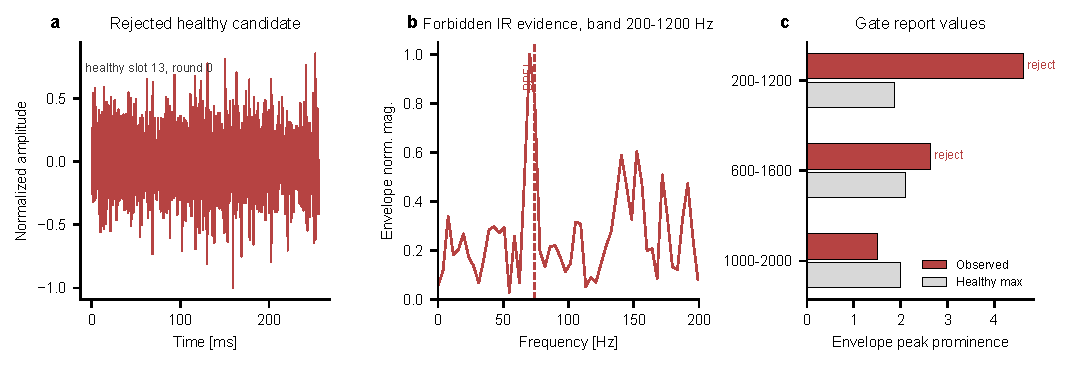
\includegraphics[width=\textwidth]{figs/failure_case.pdf}
  \caption{Complete PU LOCO failure chain. v1 and v2 are formal held-out
  evaluations; v3--v6 stop at train-only morphology, admission, sanity, or
  source-only evidence gates. The sequence prevents unsuccessful development
  stages from being reported as completed cross-condition tests.}
  \label{fig:failurechain}
\end{figure*}

\subsection{Milling boundaries}

The core milling evidence is limited to datasets with complete, auditable
protocol metadata. The private machine-tool dataset used in earlier drafts
therefore leaves the core evidence. Its speed, geometry, file-to-operation
manifest, and audited physical label mapping are incomplete, which prevents a
public reproducible portability claim.

UMich and MU-TCM define two distinct protocol stops. In the available UMich
protocol, experimental condition and process metadata are confounded with wear
labels, allowing a classifier to exploit condition identity. The current files
leave these effects entangled, so a valid formal test requires repeated
conditions or a revised acquisition design. MU-TCM v3 stops at train-only
inner validation, where only
\BreezeMUTCMPassedTests/\BreezeMUTCMRegisteredTests{} predeclared comparisons
pass; preregistration and formal held-out evaluation were therefore withheld.
Both datasets remain boundary evidence.

\section{Discussion}
\label{sec:discussion}

\subsection{The three evaluation questions define a bounded LLM contribution}

The source ablations answer the first evaluation question by establishing an
LLM recipe contribution within the matched \breeze\ pipeline. On PU, the
random-recipe-plus-verifier control produces 0 admitted slots and fails to form
a balanced pool, while random open-loop augmentation is substantially weaker
downstream. LLM recipes also exceed the fixed rule source in every registered
PU cell and every provenance-valid CWRU family.

The class-conditional diagnostics answer the second question with complementary
train-supported physical evidence. Admitted pools exhibit waveform, envelope,
PSD, band-energy, statistical-distance, and non-copy behaviour under the frozen
metrics. These measurements support admission under the declared gates while
leaving full physical truth outside their observational scope.

The downstream protocols answer the third question by locating both stable
utility and its transfer boundary. LLM recipes improve the registered PU and
provenance-valid CWRU comparisons and provide a qualified lower-shot Berkeley
advantage. Their extra value converges with the rule recipe at ten Berkeley
shots, while PU LOCO remains unsuccessful across six predeclared stages.

Together, these answers position \breeze\ as a train-calibrated control layer
around a structured black-box proposal source. This operating point supports
deployments that require inspectable admission records and bounded resampling
without training a new target generator.

\subsection{Physical admission evidence versus physical truth}

Train-calibrated gates provide auditable physical evidence within a finite set
of observables. A candidate can satisfy RMS, PSD, and envelope gates while
missing load-path, transfer-function, non-stationary, or degradation
mechanisms; a rare real sample can likewise fall outside a finite training
boundary. \breeze\ therefore reports class-wise distances, downstream tests,
and negative transfer results alongside gate pass rates. A pass means
``admissible under the declared training-calibrated gates,'' not proof of
membership in the full real distribution.

Matched source controls partially address the circularity created by shared
renderer and verifier kinematics. Rule, random, and LLM sources all encounter
the same renderer and physical checks, yet the LLM source consistently forms
the useful admitted pools in the registered PU comparisons. Further reduction
of circularity requires external expert scoring, independent physical
observables absent from the prompt, and new condition-disjoint datasets.

\subsection{Reproducibility and remaining blockers}

The repository supports replay from archived recipes through reported
statistics. It stores split manifests, prompts, recipe JSON, local renderer
seeds, waveform hashes, per-gate reports, pool manifests, seed-level classifier
rows, registered tests, and table-generation assertions. Long-running
pipelines are append-only or checkpoint-resumable. Frozen CSV/NPZ artifacts
generate every reported number, and NA explicitly marks an unavailable pool.

Two provenance and baseline blockers remain. The original PU archive omits the
provider version and provider-side sampling seed, so exact replay begins from
the archived recipes instead of the original LLM response. Completed formal
TimeGAN/DDPM and additional diagnostic-backbone comparisons are also
unavailable, which keeps state-of-the-art and universal classifier claims
outside the supported scope. Future work should complete those matched
baselines, repeat the protocol with at least one non-CNN diagnostic backbone,
and preregister a new PU cross-condition representation before accessing
held-out outcomes.

\section{Conclusion}
\label{sec:conclusion}

\breeze\ separates LLM recipe proposal, fixed seeded rendering,
train-calibrated physical admission, and downstream diagnosis. Across the
frozen public protocols, LLM recipes outperform matched controls on PU and
CWRU, provide a qualified lower-shot Berkeley benefit, and produce inspectable
physical diagnostics and gate records. The supported scope is training-free,
physics-verified admission for the stated few-shot tasks; zero-data diagnosis,
formal guarantees, PU cross-condition generalization, and universal generator
superiority remain outside it.

\section*{Data and code availability}

The release package connects each reported result to public data and frozen
evidence. PU and CWRU are public benchmarks, and Berkeley milling is available
through the NASA prognostics repository subject to its terms. The script
\texttt{scripts/build\_paper\_tables.py} generates the manuscript tables, while
\texttt{analysis/evidence\_ledger.md} and
\texttt{analysis/claim\_evidence\_map.md} enumerate numerical sources,
availability, and permitted wording. Release artifacts include gate thresholds,
per-sample pass/fail records, pool manifests, split audits, and seed-level
downstream outputs. API credentials and raw third-party datasets remain outside
the release.

\section*{Declaration of competing interest}

The authors declare that they have no known competing financial interests or
personal relationships that could have appeared to influence the work
reported in this paper.

\section*{Declaration of generative AI and AI-assisted technologies}

During preparation of this work, the authors used OpenAI Codex for code
inspection, experiment orchestration, figure and table assembly, and language
editing. The authors reviewed the evidence, verified the reported results, and
take responsibility for the manuscript.

\bibliographystyle{cas-model2-names}
\bibliography{references}

\end{document}
